\documentclass[twocolumn]{article}
\usepackage[utf8]{inputenc}
\usepackage{graphicx}
\usepackage[backend=biber]{biblatex}
\usepackage{geometry}
\usepackage{subcaption}
\usepackage[justification=centering]{caption}
\usepackage{colortbl}
\usepackage[dvipsnames]{xcolor}
\usepackage{graphics}

\geometry{margin=0.75in}
\definecolor{lightgray}{rgb}{0.9,0.9,0.9}

\addbibresource{references.bib}

\title{DeepFace: Face Generation using Deep Learning}
\author{Hardie Cate (ccate@stanford.edu)\\ Fahim Dalvi (fdalvi@cs.stanford.edu) \\ Zeshan Hussain (zeshanmh@stanford.edu)}
\date{February 17, 2016}

\begin{document}

\maketitle

\section{Introduction}
Convolutional neural networks (CNNs) are powerful tools for image classification and object detection, but they can also be used to generate images. For our project, we use CNNs in concert with other deep learning architectures to create a face generation system. Given a set of desired facial characteristics, we produce a well-formed face that matches these attributes. Potential facial characteristics fall within the general categories of raw attributes (e.g., big nose, brown hair, etc.), ethnicity (e.g., white, black, Indian), accessories (e.g. sunglasses, hat, etc.), and even emotions. In our face generation system, we fine-tune a convolutional network pre-trained on faces to create a binary classification system for the potential facial characteristics. We then use this CNN with various other deep learning architectures we are considering. Our face generation system has many potential uses, including identifying suspects in law enforcement settings.

\section{Related Work}
Work surrounding generative models for deep learning has mostly been in developing graphical models, autoencoder frameworks, and more recently, generative recurrent neural networks (RNNs). Specific graphical models that have been used to learn generative models of data are Restricted Boltzmann Machines (RBMs), an undirected graphical model with connected stochastic visible and stochastic hidden units, and their generalizations, such as Guassian RBMs. Srivastava and Salakhutdinov use these basic RBMs to create a Deep Boltzmann Machine (DBM), a multimodal model that learns a probability density over the space of multimodal inputs and can be effectively used for information retrieval and classification tasks \cite{NIPS2012_4683}. Similar work done by Salakhutdinov and Hinton shows how the learning of a high capacity DBM with multiple hidden layers and millions of parameters can be made more efficient with a layer-by-layer "pre-training" phase that allows for more reasonable weight initializations by incorporating a bottom-up pass \cite{salakhutdinov2009deep}. In his thesis, Salakhutdinov also added to this learning algorithm by incorporating a top-down feedback pass as well as a bottom-up pass, which allows DBMs to better propagate uncertainty about ambiguous inputs \cite{salakhutdinov2009learning}.

Other generative approaches involve using autoencoders. The first ideas regarding the probabilistic interpretation of autoencoders were proposed by Ranzato et al.; a more formal interpretation was given by Vincent, who described denoising autoencoders (DAEs) \cite{marc2007efficient} \cite{vincent2011connection}. A DAE takes an input $\mathbf{x} \in [0,1]^d$ and first maps it, with an encoder, to a hidden representation $\mathbf{y} \in [0,1]^{d'}$ through some mapping, $\mathbf{y} = s(\mathbf{W}\mathbf{x} + \mathbf{b})$, where $s$ is a non-linearity such as a sigmoid. The latent representation $\mathbf{y}$ is then mapped back via a decoder mapping into a reconstruction $\mathbf{z}$ of the same shape as $\mathbf{x}$. The mapping is $\mathbf{z} = s(\mathbf{W}'\mathbf{y} + \mathbf{b}')$. The parameters, $\mathbf{W}$, $\mathbf{b}$, $\mathbf{b}'$, and $\mathbf{W}'$ are learned such that the average reconstruction loss between $\mathbf{x}$ and $\mathbf{z}$ is minimized \cite{deep2016tutorial}. Bengio et al. show an alternate form of the DAE: given some observed input $X$ and corrupted input $\widetilde{X}$, where $\widetilde{X}$ has been corrupted based on a conditional distribution $C(\widetilde{X}|X)$, we train the DAE to estimate the reverse conditional $P(X|\widetilde{X})$ \cite{bengio2013generalized}. With this formulation, Vincent et al. construct a deeper network of stacked DAEs to learn useful representations of the inputs \cite{vincent2010stacked}.

An alternate model has been posited by Gregor et al., who propose using a recurrent neural network architecture to generate digits. This architecture is a type of variational autoencoder, a recent advanced model that bridges deep learning and variational inference, since it is comprised of an encoder RNN that compresses the real images during training and a decoder RNN that reconstitutes images after receiving codes \cite{gregor2015draw}. 

Finally, another approach for estimating generative models is via generative adversarial nets \cite{gauthier2014conditional} \cite{goodfellow2014generative}. In this framework, two models are simultaneously trained: a generative model $G$ that captures the distribution of the data and a discriminative model $D$ that estimates the probability that a sample came from the training data rather than $G$. $G$ is trained to maximize the probability that $D$ makes a mistake. 


\section{Datasets}
\begin{figure}[h]
    \centering
    \begin{subfigure}[b]{0.3\linewidth}
        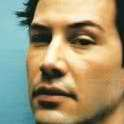
\includegraphics[width=\linewidth]{images/dataset/Keanu_Reeves_308}
        \label{fig:keanu}
    \end{subfigure}
    \hfill
    \begin{subfigure}[b]{0.3\linewidth}
        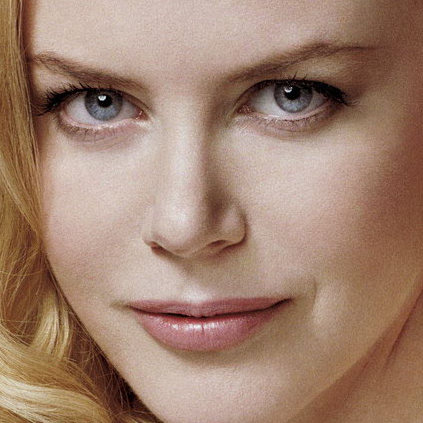
\includegraphics[width=\linewidth]{images/dataset/Nicole_Kidman_386}
        \label{fig:nicole}
    \end{subfigure}
    \hfill
    \begin{subfigure}[b]{0.3\linewidth}
        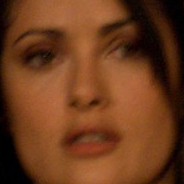
\includegraphics[width=\linewidth]{images/dataset/Salma_Hayek_184}
        \label{fig:morgan}
    \end{subfigure}
    \caption{Variations in lighting conditions and camera angles}\label{fig:dataset}
\end{figure}
We are currently using the PubFig dataset \cite{dataset}, which is a collection of faces from public photos of 200 individuals. The dataset includes 58K images scraped from various sources on the internet, and bounding boxes around the face for each of these images. However, to avoid copyright issues, the authors provide links to the images, instead of hosting the images themselves. After collecting the dataset, we now have around 28K images. The missing images include those that do not exist at the given links, those that have changed and a few that had incorrect bounding boxes for the faces.

Since these images are scraped from public photographs, there are several variations in faces we will work with. Most faces are frontal, while some are at a slight angle. There is also a wide spectrum of lighting conditions in the dataset. 

For each image in the dataset, we also have a list of 73 attributes including gender, eye color, face shape and ethnicity. Some of these attributes are dependent on each other. For example, only one of the attributes within \emph{Black Hair}, \emph{Blond Hair} and \emph{Brown Hair} is positively labelled for each individual. 

\subsection{Preprocessing}
The dataset contains real values for each of the 73 attributes provided. However, the authors mention that these values have no meaning in the absolute sense. Most of the valuable information is contained in the sign of these values, indicating the presense or absence os each of these attributes. Hence, we first convert the entire label set into a binary matrix, where positive values are mapped to one and negative values to zero. This helps us reduce the problem to a classification task, specifically a multi-label classification problem. 
\section{Technical Approach}
Our approach to the problem is two-fold. First, we train a CNN to be used in a classification system that identifies facial characteristics in existing images. Second, we use this network to generate images from a set of characteristics using one of several techniques. One possible technique is to use a variational autoencoder structure consisting of RNNs while another potential technique is to use generative adversarial nets. 


\subsection{Architecture}
\begin{figure}[h]
    \centering
    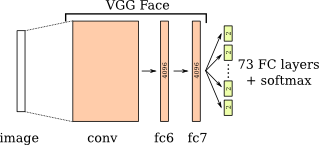
\includegraphics[width=\linewidth]{images/arch}
    \label{fig:arch}
    \caption{Baseline architecture}
\end{figure}
As a baseline for the first part of our approach, we decided to use the VGG Face CNN descriptor \cite{vggfacenet}, a CNN trained to perform face recognition on 2622 individuals. We first replace the model's final fully connected layer (fc8) with 73 smaller fully connected layers for each of the attributes. Each of these smaller fully connected layers is connected to its own softmax layer to essentially create 73 binary classifiers. 

For the second part of our approach, we propose using an extension of the variational encoder RNN architecture presented by Gregor et al as our primary candidate architecture. Specifically, we will maintain an encoder network, whose enacted function is represented by $RNN^{enc}$, and a decoder network, $RNN^{dec}$, both of which emit a hidden vector $h_t$ at time step, $t$. However, for each input image $x$, $c_o$, $h_o^{enc}$, and $h_o^{dec}$ will be initialized to be a form of the resultant fully connected layer output of the CNN architecture described above. Thus, we are essentially plugging in the trained CNN above to the RNN variational-encoder architecture. We hypothesize that this framework will generalize better, since it will learn more useful representations of the inputs given the pre-trained model.

\section{Experiments and Analysis}
Since we are fine-tuning a pretrained network for our baseline, we first decide whether or not we want to backpropagate our changes into the pretrained part of the network and the amount. One strategy we employ is to perform a forward pass on the pretrained part of the network using our dataset, and plot the fc7 layer activations in space to detect clustering.
\begin{figure}[h]
    \centering
    \hfill
    \begin{subfigure}[b]{0.49\linewidth}
        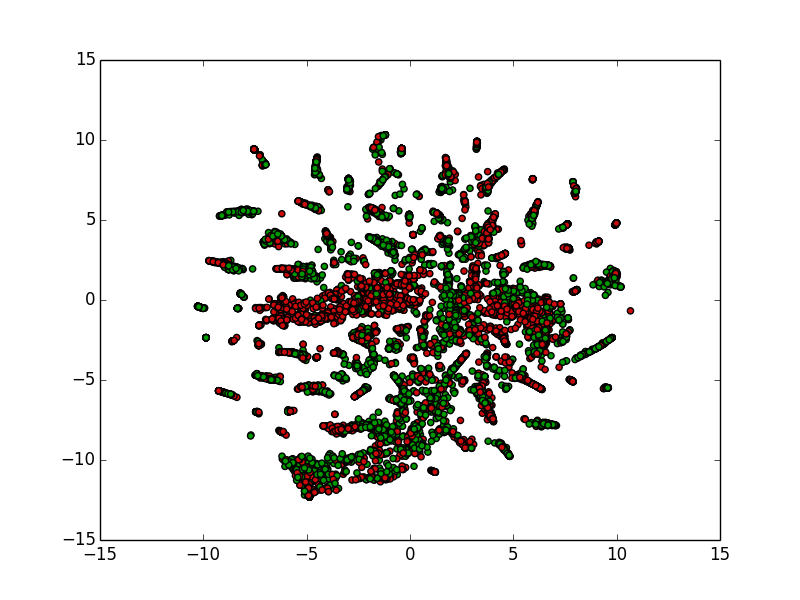
\includegraphics[width=\linewidth]{images/analysis/17}
        \label{fig:keanu}
        \subcaption{sunglasses}
    \end{subfigure}
    \hfill
    \begin{subfigure}[b]{0.49\linewidth}
        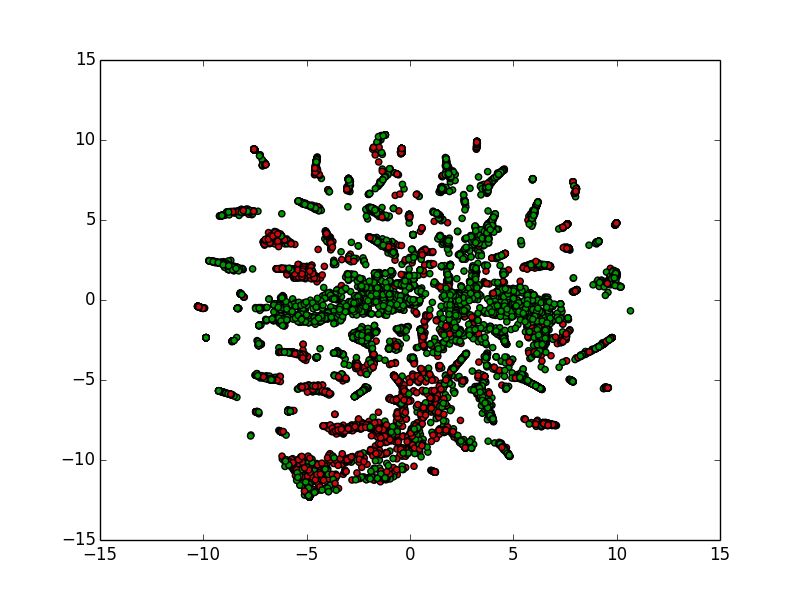
\includegraphics[width=\linewidth]{images/analysis/34}
        \label{fig:nicole}
        \subcaption{gray hair}
    \end{subfigure}
    \hfill
    \caption{2D representation of FC7 feature space}
    \label{fig:analysis}
\end{figure}

We note that for certain attributes like \emph{sunglasses}, the pretrained network features are overlapping and do not form distinctive clusters. On the other hand, for attributes like \emph{gray hair}, the pretrained network features form clusters. This is expected, since features like gray hair are indicative of a person's face, but sunglasses are not. However, this does show that there is a need for us to backpropagate our losses into the pre-trained weights.

We are also running experiments to see if we need shared fully connected layers after fc7 that we need to train from scratch for better performance.
% \subsection{Experiments}
% \subsection{Results}
% \subsection{Analysis}
%\section{Conclusions and Future Work}
\section{References}
\printbibliography[heading=none]
\end{document}

